\documentclass[11pt]{article}
\usepackage[margin=1in]{geometry}
\usepackage[T1]{fontenc}
\usepackage{lmodern}
\usepackage{amsmath,amssymb,amsthm}
\usepackage{graphicx,booktabs,enumitem}
\usepackage[dvipsnames]{xcolor}
\usepackage[authoryear,round]{natbib}
\usepackage{xurl}
\usepackage[colorlinks=true,linkcolor=blue!50!black,citecolor=blue!50!black,urlcolor=blue!50!black]{hyperref}
\usepackage{setspace}
\setstretch{1.15}
\newtheorem{proposition}{Proposition}
\bibliographystyle{plainnat}

\title{Tied Hands, Turned Around:\\[2pt] \large Trade Protection, Trade Demands, and Credible Commitment in NHL Contracts}
\author{Dubya\thanks{Data, code and replication files: \texttt{nhl-trade-protection/} in the accompanying repository. All data were collected from public sources on 30 October 2026. Comments welcome.}}
\date{30 October 2026}

\begin{document}
\maketitle

\begin{abstract}\noindent
No-trade and no-movement clauses are meant to protect NHL players from their teams. This paper shows how, once a protected player asks to leave, the clause is turned against the team that granted it. Drawing on international-relations bargaining theory (commitment problems, tying hands, veto players and audience costs), I model the exit of a protected player as a sale in which the player chooses the set of eligible buyers. The incumbent's return rises with the number of approved destinations but with sharply diminishing returns: in a calibrated example, a ten-team no-trade list costs the seller about 3 per cent of the competitive price, and a three-team approved list nearly half. Publicity and narrow lists are complements. Going public destroys the seller's outside option only when few buyers are approved. Using a new dataset of every NHL contract-season and trade from 2005--06 to 2026--27, assembled from the records of 7,965 players, I document that protected contracts in force nearly doubled after 2013--14, to 306, and now account for 49 per cent of cap dollars and 77 per cent of star contracts. On deals already signed, 45 per cent of the projected 2027--28 league-wide cap is committed to players holding a veto. Protection roughly halves a player's annual probability of being traded, but carries no detectable wage discount. A coded set of 25 star exits from 2008 to 2026, including the 2026 wave of Tkachuk, Larkin, Hellebuyck and Nurse, is consistent with the model: public-from-the-start demands returned about a third of the draft capital of those that began privately. I conclude with contract-design implications, chief among them minimum approved-list sizes and clauses that decay over time.

\medskip\noindent\textbf{Keywords:} no-trade clause; credible commitment; audience costs; veto players; bargaining; NHL; contract design
\end{abstract}

\section{Introduction}\label{sec:intro}

In the twelve months before this paper was written, five established stars of the National Hockey League left their teams or tried to, four of them members of the same American Olympic roster. Quinn Hughes, Vancouver's captain, told the Canucks he would not sign another contract and was traded to Minnesota in December 2025 \citep{espn_hughes,cbs_hughes}. Brady Tkachuk, Ottawa's captain, asked to be traded and was sent to Florida on the second night of the 2026 draft \citep{cp24_tkachuk,fourthperiod_tkachuk}. Dylan Larkin, Detroit's captain, asked out on 4 June 2026. He spent the summer and autumn in limbo, was stripped of the captaincy, and was suspended without pay on 29 October \citep{wilx_larkin,nhl_larkin,cod_larkin_suspended}. Connor Hellebuyck, the league's best goaltender, asked Winnipeg for a trade privately, made the request public in August, sat out training camp, and was traded to New Jersey on 23 October \citep{nhl_hellebuyck_suspended,nhl_hellebuyck_trade}. Darnell Nurse asked Edmonton to trade him and was in San Jose within three weeks \citep{cp24_nurse,score_nurse}. Four of these players had won Olympic gold together in Milan in February \citep{nhl_olympics,dfo_trend}. On 1 October the commissioner, Gary Bettman, said the league had ``gotten past the way no-trade clauses were originally intended'' \citep{dfo_bettman}. The players' association called the remark an attack on negotiated rights \citep{tsn_hainsey}.

Bettman's remark points to a puzzle. A no-trade clause (NTC) or no-movement clause (NMC) is a right that protects a player against his employer. It is usually paired with a long-term contract, and the pair is understood as a mutual commitment: the player gets stability and the team gets his prime years. Yet when a protected player asks to be traded, the clause works \emph{against the team that granted it}. It gives the player a veto over destinations, which shrinks the set of buyers to the handful of teams the player names. It signals to every buyer that the seller must sell. And when the request is public, it removes the seller's last bargaining chip, the threat to keep the player. As Ottawa's general manager put it after the Tkachuk trade, the clause ``changes how the transaction works'' and ``it's not like he was available to every team in the league'' \citep{yahoo_staios}.

This paper argues that this reversal is best understood with the tools of international-relations bargaining theory, and that it has measurable consequences. Asking for a trade does not breach the clause. The clause is the player's right, and waiving it is entirely his choice. What breaks is the \emph{implicit} commitment of the long-term deal: the understanding that the player who accepted security will supply loyalty in return. That commitment is not self-enforcing \citep{fearon1995,powell2006}. When it fails, the clause turns from a shield into a lever. A trade request ties the team's hands \citep{schelling1960,fearon1997}. The clause makes the player a veto player with agenda-setting power over the set of buyers \citep{tsebelis2002}. And publicity creates audience costs that make the player's exit credible and the team's resistance incredible \citep{fearon1994,tomz2007}.

I make three contributions. The first is a simple formal model, built from auction theory and Nash bargaining, that shows how clause scope, publicity and delay interact. The incumbent's expected return rises with the number of destinations the player approves, but with sharply diminishing returns. In a calibrated example, a ten-team no-trade list costs the seller about three per cent of the competitive price, while a three-team approved list costs nearly half. Audience costs and veto scope are \emph{complements}: going public hurts the seller only when the approved list is short. The model also explains why teams sometimes treat unprotected players as if they held a clause (informal protection), why narrow lists produce stalemates, and why protection should be priced into contracts.

The second contribution is a new league-wide dataset. I assembled it from the contract and transaction records of 7,965 players on CapWages \citep{capwages}, a public successor to the defunct CapFriendly. It covers every contract-season from 2005--06 to 2026--27, plus commitments already signed through 2031--32, and every trade that moved a player under contract. The data show a structural shift. The number of protected contracts in force has nearly doubled since 2013--14, from 158 to 306. Protected contracts now account for 49 per cent of all cap dollars and 77 per cent of contracts worth at least 7.5 per cent of the cap. On contracts already signed, protected deals will make up 67 per cent of committed cap dollars in 2028--29 and 80 per cent in 2030--31. The share of trades that involve a protected player has risen from about one in six during the 2010s to more than one in four since 2023--24. Protected players are traded far less often than comparable unprotected players. Yet I find no evidence that teams extract a wage discount in return. Conditional on production, age and term, protected contracts pay about nine per cent \emph{more}. Protection is not priced as the model says an efficient market would price it.

The third contribution is a twenty-year case dataset of 25 star exits and refusals, coded by clause type, publicity, approved-destination count, time to resolution and return. The cases are too few and too heterogeneous for causal claims, and I make none. They are consistent with the model on the dimensions it emphasises. Demands that were public from the start brought back roughly a third of the draft capital of demands that began privately. And the longest stalemates (Luongo, Tarasenko, and now Larkin) occurred where an approved list was short or a contract was long.

The argument matters beyond hockey. Veto rights granted to protect a weaker party can be turned into instruments of extraction once the underlying relationship sours. Examples include minority-shareholder protections, alliance guarantees, and consent requirements in coalition agreements. Hockey offers an unusually clean setting in which to watch this happen, because contracts, clauses and transactions are public, and the bargaining is narrated in real time by the parties themselves.

The rest of the paper proceeds as follows. Section~\ref{sec:background} describes the institutions. Section~\ref{sec:theory} sets out the theoretical mechanisms, and Section~\ref{sec:model} formalises them. Section~\ref{sec:empirics} presents the league-wide evidence, and Section~\ref{sec:cases} the cases. Section~\ref{sec:implications} draws out implications for contract design, and Section~\ref{sec:conclusion} concludes.

\section{Institutional Background}\label{sec:background}

\paragraph{The rule.} Article 11.8 of the collective bargaining agreement (CBA) between the NHL and the NHLPA allows the contract of any player who is a Group 3 unrestricted free agent to ``contain a no-Trade or a no-move clause'' \citep{cba2013}. A Group 3 free agent is a player with seven accrued seasons or aged 27 or older. A clause may be negotiated earlier only if it does not take effect until the player reaches that status. If the player is traded before the clause takes effect, the acquiring team is not bound unless it agrees in writing. Once in force, the clause stays in the contract after a trade. An NMC is broader than an NTC: it prevents ``the involuntary relocation of a Player, whether by Trade, Loan or Waiver claim,'' but it cannot restrict buyouts (Article 11.8(c)).

\paragraph{Contract practice.} The CBA does not define partial clauses, so the parties have invented them. A \emph{modified} NTC typically lets the player submit a list of teams to which he may not be traded (a no-trade list), or a list of teams he would accept (a trade list), often with a list size that changes over the life of the contract. A typical modern star contract combines several layers: an NMC for the first years, converting on a fixed date to a modified NTC whose list shrinks as the contract ages. Adam Lowry's Winnipeg extension, for instance, carries an NMC through June 2028 and then converts to a modified NTC with a five-team, and later a ten-team, trade list (CapWages contract notes). The median modified list in the data blocks ten teams. In the paper's notation, the player may block $k\approx10$ of the 31 other teams.

\paragraph{Term limits and the cap.} The 2005 CBA introduced the salary cap and set no maximum contract term, which produced a wave of very long, front-loaded deals. The 2013 CBA capped terms at eight years for a team re-signing its own player and seven otherwise. The 2025 agreement, effective 16 September 2026, cuts these to seven and six years and tightens salary variance \citep{dfo_dfo_cba}. The 2026 free-agency period was therefore the last under the old maximums, and teams hurried to register eight-year deals before the deadline. The cap was flat at \$81.5 million from 2019--20 through 2021--22 because of COVID-19. It has since risen sharply, to \$95.5 million in 2025--26 and \$104 million in 2026--27.

\paragraph{Why NMCs bind beyond trades.} For the 2017 Vegas and 2021 Seattle expansion drafts, players with an NMC in effect ``must be protected (and will be counted toward their club's applicable protection limits)'' \citep{nhl_expansion_rules}. Clauses therefore have real costs beyond trade demands, which the model captures as $C_0(k)$.

\paragraph{The comparison.} No-trade rights are far rarer in other North American leagues. NBA contracts almost never include them; one recent count puts the number of NBA players ever to hold one at about ten \citep{gerstle2025}. Major League Baseball has a statutory ``10-and-5'' right and occasional negotiated clauses. \citet{pedacehall2012} find that MLB players trade some salary for no-trade protection. In the NBA, star trade demands are frequent, but the player has no formal veto, so the resulting leverage is informal and comes mainly through threats not to re-sign. That is exactly the mechanism of Proposition~\ref{prop:informal}. Hockey is the league in which formal veto rights are most widespread, which makes it the natural laboratory.

\paragraph{Related work.} The economics of player mobility is old \citep{rottenberg1956,kahn2000,fortquirk1995}, and hockey salaries have been studied extensively \citep{idsonkahane2000,cyrenne2013,kahane2024}. \citet{fumarco2024} study strategic behaviour around NHL mobility restrictions, and \citet{marburger2009} asks why player trades dominate cash sales. As far as I can find, however, no peer-reviewed study estimates the price of NTCs or NMCs in the NHL, the league where they are most common, and none models trade demands as a strategic credibility problem. The closest descriptive work is \citet{hockeygraphs2021}. This paper aims to fill that gap.

\section{Theory: Four Mechanisms from International Relations}\label{sec:theory}

The bargaining literature in international relations is a natural home for the trade-request problem. It studies how parties with conflicting interests settle disputes when commitments cannot be enforced by a third party, when private information gives each side a reason to misrepresent its resolve, and when public statements change what each side can later accept. All three conditions hold here. I draw on four mechanisms.

\subsection{The commitment problem}

\citet{fearon1995} identifies commitment problems as one of three rationalist explanations for costly bargaining failure. Two parties may prefer a negotiated settlement to conflict, yet fail to reach one because one side cannot credibly promise not to exploit a future shift in power. \citet{powell2006} generalises the point: large, rapid shifts in the distribution of power make today's bargains worthless tomorrow.

A long-term NHL contract has the same structure. The team commits money, cap space and roster construction for six, seven or eight years. In return, the player promises his prime seasons. The team's side of the bargain is legally enforceable, because the salary is guaranteed and the clause binds. The player's side is not. Labour law and the CBA guarantee that he will be paid, but nothing guarantees that he will want to stay, and the things that matter most to the team (effort, leadership and willingness to sign the next contract) cannot be written into a contract. In the language of incomplete contracts \citep{hartmoore1988,hartmoore1990}, the player retains residual control over his own engagement. The player's commitment is therefore not \emph{self-enforcing}. When his outside option improves or his value of staying falls (a rebuild, a coaching change, a family move), the bargain is renegotiated in fact even though it is not renegotiated in law.

This is what the paper means by \emph{defection from the implicit commitment}. A trade request does not breach the NTC or NMC. The clause is a right the player holds, and waiving it is entirely his choice. What breaks is the unwritten half of the long-term deal.

\subsection{Tying hands, turned around}

\citet{schelling1960} observed that the power to bind oneself is the power to constrain an adversary. A negotiator who can credibly eliminate his own options forces the other side to accommodate. \citet{fearon1997} formalises this as \emph{tying hands}: a signal is credible if sending it and then backing down is costly.

In the standard story, the clause ties the team's hands for the player's benefit: the team cannot move him. The twist here is that a trade request reverses the direction. Once the player announces that he wants out, the team's hands are tied in the market for his services. Every rival general manager now knows that the incumbent must sell, so the incumbent's implicit threat to keep the player loses credibility. The clause that was meant to protect the player against the team becomes, in the hands of a player who wants to leave, a weapon against the team.

\subsection{Veto players and agenda control}

\citet{tsebelis2002} shows that adding a veto player shrinks the set of feasible policy changes (the ``winset''). A player with a full NMC is a veto player over every possible transaction. When he demands a trade, he does not merely accept or reject offers. He sets the agenda by naming the teams he will accept. That narrows the field of buyers, sometimes to one. The NHL's own language reflects this: Ottawa's general manager said Brady Tkachuk's clause ``changes how the transaction works'' and that the process was ``pointed at one team at the end'' \citep{cp24_tkachuk}. In auction terms, the veto converts a competitive sale into a bilateral negotiation, and \citet{bulowklemperer1996} show that competition among buyers is worth more to a seller than almost any amount of negotiating skill. The surplus the seller loses does not go to the player. It goes to the favoured buyer.

\subsection{Audience costs}

\citet{fearon1994} argues that leaders who make public threats incur \emph{audience costs} if they back down, and that these costs make public threats more credible than private ones. \citet{tomz2007} provides experimental evidence for such costs, while \citet{snyderborghard2011} question how often they bind. A public trade request is a public threat. It raises the player's own cost of reconciling with the team (fans, teammates and media will treat a reversal as weakness or insincerity) and therefore makes his exit credible. It also destroys the team's ability to bluff. Privately, a team can tell suitors that it is happy to keep the player and see whether the situation improves. Once the request is public, that claim is no longer believable. Connor Hellebuyck's request, private for months and then confirmed publicly in August 2026, is the clearest recent example \citep{thw_larkin_hellebuyck,br_hellebuyck}.

\subsection{Holdup and sunk costs}

Two further ideas complete the toolkit. First, the trade-request problem is a form of the \emph{holdup} studied in transaction-cost economics \citep{kca1978,williamson1979,williamson1985}. The team makes relationship-specific investments (cap commitments, roster construction, a marketing identity built around the player) whose value depends on the player's continued cooperation, and the clause lets that quasi-rent be appropriated ex post. The holdup here is unusual because the party that appropriates the rent is not the counterparty: the player gets his preferred destination, while the money goes to the acquiring team. Second, decision makers are prone to honour sunk costs \citep{arkesblumer1985,staw1976}, and sports organisations are no exception \citep{stawhoang1995,camererweber1999}. A team that has just committed \$70 million to a captain may wait in the hope that he changes his mind, even when the expected value of waiting is negative. Detroit's handling of Dylan Larkin's 2026 request illustrates the temptation.

\section{A Model of Protected Exit}\label{sec:model}

The model is deliberately simple. Its job is to make the four mechanisms precise, show how they interact, and generate propositions that can be compared with the cases and the data. Intuition comes first in each step; proofs are in Appendix~\ref{app:proofs}.

\subsection{Setup}

\paragraph{Players.} An incumbent team $T$ holds the contract of a protected player $P$. There are $N$ other teams, the potential acquirers $A_1,\dots,A_N$ ($N=31$ in today's league). Acquirer $i$ values $P$ at $v_i$, drawn independently from a distribution $F$ on $[0,\bar v]$ with positive density. $T$ does not observe the $v_i$.

\paragraph{Stage 1: contract.} $T$ and $P$ agree on a wage $w$ and a protection scope $k\in\{0,1,\dots,N\}$, the number of teams $P$ may block. A full NTC or NMC is $k=N$, a modified clause with a ten-team no-trade list is $k=10$, and no clause is $k=0$.

\paragraph{Stage 2: shock.} $P$'s value of staying, $u_{\text{stay}}$, is hit by a shock: the team enters a rebuild, the coach changes, family circumstances change. If $u_{\text{stay}}$ falls below the value of leaving, $u_{\text{out}}$, $P$ demands a trade. This happens with probability $q$, which is common knowledge at Stage 1.

\paragraph{Stage 3: signal.} $P$ chooses whether to make the demand privately or publicly, $s\in\{\text{priv},\text{pub}\}$. Going public costs $P$ an audience cost $c_P$ if he later reconciles with $T$, and it makes the demand common knowledge among acquirers.

\paragraph{Stage 4: sale.} $P$ approves a set of destinations of size $m$. Under a clause of scope $k$, $m\ge N-k$; with a full clause, $P$ chooses $m\ge 1$ freely. $T$ either sells $P$ to an approved acquirer or keeps him. If $T$ keeps $P$, it receives the \emph{retention value}
\begin{equation}\label{eq:R}
R_s \;=\; \lambda_s V + (1-\lambda_s)\,V_d,
\end{equation}
where $V$ is the value of a recommitted player, $V_d<V$ is the value of a disgruntled one (lower effort, locker-room friction, the certainty of losing him at the next opportunity), and $\lambda_s$ is the probability that the relationship is repaired. Because a public demand raises $P$'s own cost of backing down, $\lambda_{\text{pub}}<\lambda_{\text{priv}}$, and therefore $R_{\text{pub}}<R_{\text{priv}}$. The audience cost works by tying the \emph{player's} hands, which in turn lowers the \emph{team's} outside option.

\paragraph{The sale mechanism.} If $m\ge2$, $T$ runs a competitive process among approved acquirers with reserve $R_s$. This is equivalent to an English auction in which $T$ keeps $P$ if no bid exceeds $R_s$. If $m=1$, competition is impossible, and $T$ and the single acquirer split the gains from trade by Nash bargaining, with $T$'s bargaining weight $\beta\in[0,1]$ and disagreement point $R_s$. Writing $v_{(j:m)}$ for the $j$-th highest of $m$ valuations, $T$'s expected return is
\begin{equation}\label{eq:Pi}
\Pi(m,R) \;=\;
\begin{cases}
R + \beta\,\mathbb{E}\big[(v-R)^+\big] & m=1,\\[3pt]
\mathbb{E}\big[\max\{v_{(2:m)},\,R\}\big] & m\ge2.
\end{cases}
\end{equation}
For $m\ge2$, the second-highest approved valuation sets the price unless the reserve binds. If the highest valuation falls below $R$, $T$ keeps $P$ and receives $R$. These cases combine into the single expression $\mathbb{E}[\max\{v_{(2:m)},R\}]$.

\subsection{How the veto transfers surplus}

\begin{proposition}[Veto scope]\label{prop:veto}
(i) For $m\ge 2$, $\Pi(m,R)$ is strictly increasing in $m$, and therefore strictly decreasing in clause scope $k$ whenever the clause binds ($m=N-k$). (ii) The marginal value of an additional approved destination vanishes as $m$ grows and, for uniform $F$, is strictly decreasing in $m$: the first few names on a list are worth far more than the last. (iii) Moving from a competitive sale to bilateral bargaining ($m=2\to1$) lowers $T$'s return unless $T$ is an unusually strong bargainer. Under $F=U[0,1]$ and $R=0$, $\Pi(2)>\Pi(1)$ if and only if $\beta<2/3$.
\end{proposition}

\noindent\emph{Intuition.} With more approved bidders, the second-highest valuation is stochastically larger, so the price rises. Order statistics flatten out quickly, so most of this effect comes from the first handful of buyers. Table~\ref{tab:model} gives the numbers for the uniform case with $N=31$. A ten-team no-trade list ($m=21$) costs the incumbent about three per cent of the competitive price ($0.909$ against $0.937$). A three-team list of the kind Larkin reportedly submitted ($m=3$) costs nearly half ($0.507$). A single-destination veto leaves $T$ with roughly what it can extract in a bilateral negotiation in which its threat to walk away is weak. The surplus $T$ loses is not captured by $P$, who gets only his choice of destination. It goes to the acquirer. This is the formal content of the intuition that ``the other team knows the player wants out so they can rip them off.''

\subsection{Why going public hurts the incumbent}

\begin{proposition}[Audience costs]\label{prop:audience}
(i) $\Pi(m,R)$ is strictly increasing in $R$, with $\partial\Pi/\partial R = G_{(2:m)}(R)$ for $m\ge2$, where $G_{(2:m)}$ is the CDF of $v_{(2:m)}$, and $\partial\Pi/\partial R=1-\beta(1-F(R))$ for $m=1$. Hence a public demand, which lowers $R$ from $R_{\text{priv}}$ to $R_{\text{pub}}$, lowers $T$'s return. (ii) For $m\ge2$, the loss from going public is strictly decreasing in $m$, so veto scope and audience costs are complements. The loss is larger still at $m=1$ whenever $\beta\le 1-F(R_{\text{priv}})$.
\end{proposition}

\noindent\emph{Intuition.} The retention value matters only when it is the binding alternative to a sale, that is, when competition among buyers is weak. With many approved bidders, the second-highest bid almost always exceeds any plausible retention value, and the team's ability to bluff is irrelevant. With one or two approved bidders, the retention value is the team's main source of leverage, and a public demand destroys it. In the uniform example, a fall in $R$ from $0.20$ to $0.05$ costs $T$ $0.084$ when $m=1$, $0.035$ when $m=2$, $0.007$ when $m=3$, and nothing at all once $m\ge5$ (Table~\ref{tab:model}).

A refinement sharpens this. If bilateral bargaining is modelled as Rubinstein alternating offers with an outside option, the \emph{outside-option principle} \citep{rubinstein1982,bss1989} implies that $T$'s payoff is $\max\{\beta^\ast v, R\}$, where $\beta^\ast$ is its Rubinstein share. A public demand then hurts only those teams whose threat to keep the player was binding, that is, contenders and teams whose identity is built around the player. Teams that would have sold anyway lose nothing from publicity.

\paragraph{Why players go public.} Going public is costly for the player too, so why do it? Let $\tau_s$ be the probability that $T$ sells, which falls with $R_s$ because $T$ keeps $P$ when no approved bid exceeds the reserve. $P$ goes public if and only if
\begin{equation}\label{eq:public}
(\tau_{\text{pub}}-\tau_{\text{priv}})\,(u_{\text{out}}-u_{\text{stay}}) \;\ge\; c_P\,\lambda_{\text{pub}}.
\end{equation}
Publicity is a commitment device. It ties the player's hands so that the team's do not have to be tied for it. The condition is most likely to hold after a private request has stalled, when $\tau_{\text{priv}}$ is low because $T$ believes it can wait. This is the sequence observed in Winnipeg in 2026: a private request early in the offseason, then public confirmation in late August.

\subsection{Delay and the sunk-cost temptation}

Suppose $T$ can wait one period. With probability $\rho$ the shock reverses and $P$ recommits, worth $V$ (normalised to 1). Otherwise $T$ sells next period. At that point the clause may have loosened ($m'\ge m$; many contracts convert an NMC into a modified NTC on a fixed date), the player's value has decayed, and payoffs are discounted by $\delta$.

\begin{proposition}[Delay]\label{prop:delay}
$T$ prefers to wait if and only if $\rho + (1-\rho)\,\delta\,\Pi(m',R') > \Pi(m,R)$. Waiting is therefore more attractive (a) when the current approved set is small, because $\Pi(m,R)$ is low, (b) when the clause is scheduled to loosen, because $m'>m$, and (c) when the team believes reconciliation is likely (high $\rho$).
\end{proposition}

\noindent\emph{Intuition.} A narrow list does not just lower the price. It also lowers the opportunity cost of waiting, so the model predicts stalemates exactly where clauses are tightest. Part (c) is where behaviour enters. A team that has just signed the player to an eight-year deal and named him captain has every psychological reason to overestimate $\rho$ \citep{arkesblumer1985,stawhoang1995}. Overestimating $\rho$ produces delay that the fundamentals do not justify.

\subsection{Pricing the clause ex ante}

At Stage 1, the parties anticipate the possibility of a demand. Let $B(k)$ be $P$'s private value of protection, which is increasing in $k$, and let $C(k)=q\,[\Pi(N,R)-\Pi(N-k,R)] + C_0(k)$ be $T$'s expected cost. The second term, $C_0(k)$, captures costs unrelated to demands, such as lost roster flexibility and mandatory expansion-draft protection for NMCs. Suppose wage and scope are set by generalised Nash bargaining in which $P$ receives share $\alpha$ of the surplus.

\begin{proposition}[The price of protection]\label{prop:price}
The equilibrium wage satisfies $w(k)=w(0)-\big[(1-\alpha)B(k)+\alpha C(k)\big]$, so the clause is paid for by a wage discount that is a weighted average of what the player values and what the team expects to lose. The discount, $\partial w/\partial k$, rises in absolute value with $q$. If wages cannot fall, for example because the player is already at the market maximum, a higher $q$ instead lowers the scope teams will grant.
\end{proposition}

\noindent\emph{Intuition.} Protection has a price, and it should move with the perceived probability of demands. Each publicised request that turns a clause against its team raises the $q$ that general managers apply to new contracts, so the model predicts that the 2026 wave will show up as narrower lists, shorter protection windows, more scheduled conversions from NMC to modified NTC, and more resistance to full NMCs. The salary cap adds a twist. When the cap binds, money is scarce and protection is a non-cash currency teams can still offer, so prevalence should rise when cap growth is slow. Section~\ref{sec:empirics} tests both implications.

\subsection{Informal protection without a clause}

The final proposition explains why a team can behave as if a player has a clause when he does not. Suppose that an acquirer's valuation has two parts: the value of the remaining contract term, $x_i$, and the value of extending the player, $E$. The extension value is realised only if $P$ is willing to re-sign with that team. If $P$ makes clear that he will extend only with teams in a set $A$, then acquirers outside $A$ value him at $x_i$ and acquirers inside $A$ value him at $x_i+E$.

\begin{proposition}[Informal protection]\label{prop:informal}
If $E>\bar x$, where $\bar x$ is the maximum term value, and $|A|\ge2$, then the two highest valuations always belong to approved teams, and $T$'s expected return equals $\Pi(|A|,R)$ computed on approved valuations, exactly as if $P$ held a formal clause of scope $N-|A|$. The equivalence is stronger the less term remains on the contract.
\end{proposition}

\noindent\emph{Intuition.} Near the end of a contract, what an acquirer buys is mostly the right to negotiate an extension, and that right is worth something only if the player cooperates. A star with eighteen months left therefore carries informal veto power over his destination, which is what Quinn Hughes's agent meant when he said Vancouver acted ``as if we had a no-trade clause'' \citep{dailyhive_hughes}. The corollary matters for interpretation. The formal clause has most bite precisely when many years remain, which is when the implicit commitment of the long-term deal is supposed to hold.

\subsection{Contagion}

Finally, let the player's private cost of demanding a trade fall with the number of recent successful demands by peers, $c_P = c(n)$ with $c'(n)<0$. Successful demands lower the stigma of being seen as a quitter and reveal how teams and markets respond. The probability that a given shock produces a demand is then increasing in $n$, so demands should \emph{cluster} in time and within networks of players who share information. The 2026 cluster among members of the same Olympic roster fits this prediction, although four cases cannot distinguish contagion from common shocks.

\begin{table}[t]\centering\small
\caption{Incumbent's expected return by number of approved destinations ($F=U[0,1]$, $N=31$, $\beta=0.5$)}\label{tab:model}
\begin{tabular}{rrccc}\toprule
Approved $m$ & Blocked $k$ & Private ($R=0.20$) & Public ($R=0.05$) & Loss from publicity\\\midrule
1 & 30 & 0.360 & 0.276 & 0.084\\
2 & 29 & 0.371 & 0.336 & 0.035\\
3 & 28 & 0.507 & 0.500 & 0.007\\
5 & 26 & 0.667 & 0.667 & 0.000\\
10 & 21 & 0.818 & 0.818 & 0.000\\
16 & 15 & 0.882 & 0.882 & 0.000\\
21 & 10 & 0.909 & 0.909 & 0.000\\
31 & 0 & 0.937 & 0.937 & 0.000\\
\bottomrule\end{tabular}
\begin{minipage}{0.92\linewidth}\footnotesize\vspace{4pt}
\emph{Notes:} Returns are expressed as a share of the maximum possible valuation. $R=0.20$ represents a private demand and $R=0.05$ a public one. The final column is the loss from going public. Computed by \texttt{analysis/05\_model\_numerics.py}.
\end{minipage}
\end{table}

\section{Evidence from Twenty Years of Contracts and Trades}\label{sec:empirics}

\subsection{Data}

The NHL does not publish contract terms, and the most widely used public archive, CapFriendly, closed in 2024. I rebuilt the league's contract history from CapWages \citep{capwages}, which publishes, for each player, every standard player contract with its per-season cap hit and clause status (NMC, NTC, modified NTC, modified NMC), free-text clause details, and a transaction log in which every trade carries a unique identifier. I collected the pages of all 7,965 players listed in the site's index on 30 October 2026. This yielded 12,800 contracts and 27,381 contract-seasons between 2005--06 and 2026--27, together with every season already committed under signed contracts through 2034--35. Seasons are NHL league years (1 July to 30 June). Modified-clause list sizes are parsed from the clause text. Appendix~\ref{app:data} documents the variables and every coding decision.

Two checks support the data. First, coverage: matching the contract panel to official NHL season rosters, at least 94 per cent of rostered players in every season from 2014--15 onward (and 91 per cent in 2013--14) have a contract on file. Coverage falls to 75 per cent in 2009--10 and below half before 2007--08, because the archive under-represents players who retired early in the cap era. I therefore treat 2013--14 onward as the primary sample and flag earlier seasons. Second, external validity. The trade series reproduces the NHL's official count of trade-deadline-day transactions \citep{nhl_statspack} with a correlation of 0.96 and a mean absolute error of 1.1 trades per year across the 17 seasons from 2009--10 to 2025--26. The 2026--27 clause counts (306 protected contracts, 120 of them NMCs) are close to an independent August 2026 count of 312 protected players and 111 NMCs \citep{deseret_ntc}.

The trade series counts every trade that moved at least one player under contract. It does not capture pick-only trades. A ``protected trade'' is one that moved a player whose contract carried any clause in that season. Since an in-force clause must be waived for a trade to proceed, every such trade is one the player consented to.

\subsection{The rise of trade protection}

Figure~\ref{fig:prev} and Table~\ref{tab:prev} show the trend. In 2013--14, the first season of the primary sample, 158 contracts carried some form of trade protection, about five per team. By 2026--27 the number was 306, almost ten per team. Over the same period the protected share of all cap dollars rose from 31 to 49 per cent, and the protected share of star contracts (those worth at least 7.5 per cent of the cap) rose from 62 to 77 per cent. The increase was not steady. Prevalence was flat through the late 2010s and the flat-cap years, then rose sharply from 2022--23 as the cap began to grow again. The composition shifted too: NMCs, the strongest form, grew from 68 to 120.

Two features of the trend fit the model's account of protection as a non-cash currency (Proposition~\ref{prop:price}). The first is the timing of the take-off. It began as teams emerged from the flat cap carrying long commitments, and it accelerated as the 2025 CBA's shorter term limits approached. Under those conditions protection is one of the few concessions a team can offer a star without spending cap space. The second is that the protected share of new long-term deals for established players has trended up across signing cohorts (Figure~\ref{fig:cohorts}). Among multi-year contracts worth at least five per cent of the cap signed by players aged 26 or older, the share granting a full NTC or NMC at some point rose from 45--50 per cent in 2009--13 to 74 and 82 per cent in the 2024--25 and 2025--26 cohorts.

\begin{figure}[t]\centering
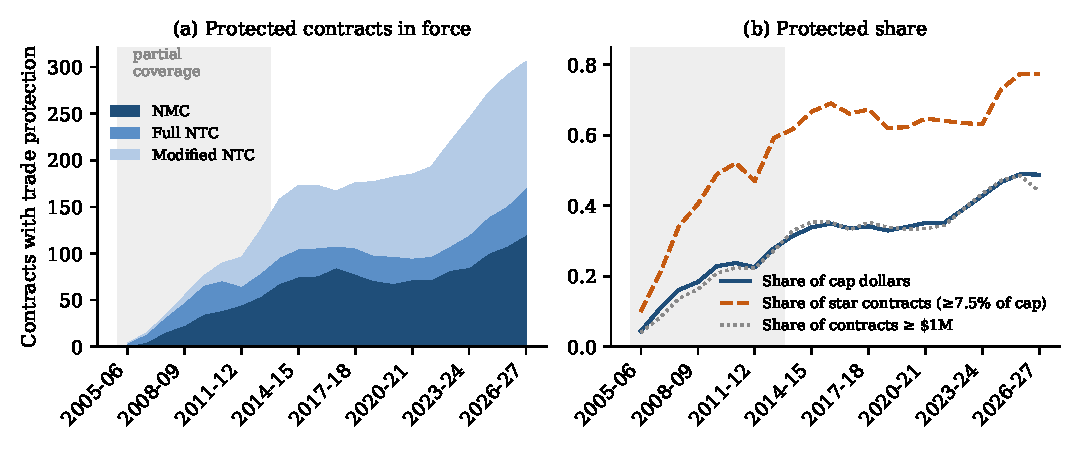
\includegraphics[width=\linewidth]{../analysis/figures/fig_prevalence.pdf}
\caption{Trade protection in force, 2005--06 to 2026--27. Shaded seasons have incomplete coverage (fewer than 90 per cent of rostered players matched to a contract). Source: author's compilation from CapWages.}\label{fig:prev}
\end{figure}

\begin{table}[t]\centering\scriptsize
\caption{Trade protection by season}\label{tab:prev}
\begin{tabular}{lrrrrrrrr}\toprule
Season & Protected & NMC & NTC & M-NTC & Per team & Share cap $ & Share stars & Median NT list\\\midrule
2009-10 & 76 & 34 & 31 & 10 & 2.5 & 0.23 & 0.49 & \\
2010-11 & 90 & 39 & 32 & 19 & 3.0 & 0.24 & 0.52 & \\
2011-12 & 96 & 45 & 20 & 31 & 3.2 & 0.23 & 0.47 & \\
2012-13 & 125 & 54 & 25 & 46 & 4.2 & 0.28 & 0.59 & 8\\
2013-14 & 158 & 68 & 28 & 62 & 5.3 & 0.31 & 0.62 & 6\\
2014-15 & 173 & 75 & 30 & 68 & 5.8 & 0.34 & 0.67 & 10\\
2015-16 & 173 & 76 & 30 & 67 & 5.8 & 0.35 & 0.69 & 10\\
2016-17 & 167 & 85 & 23 & 59 & 5.6 & 0.34 & 0.66 & 10\\
2017-18 & 176 & 78 & 28 & 70 & 5.7 & 0.34 & 0.67 & 10\\
2018-19 & 177 & 71 & 27 & 79 & 5.7 & 0.33 & 0.62 & 10\\
2019-20 & 182 & 68 & 29 & 85 & 5.9 & 0.34 & 0.62 & 10\\
2020-21 & 185 & 72 & 23 & 90 & 6.0 & 0.35 & 0.65 & 10\\
2021-22 & 193 & 72 & 25 & 96 & 6.0 & 0.35 & 0.64 & 10\\
2022-23 & 220 & 82 & 26 & 112 & 6.9 & 0.39 & 0.63 & 10\\
2023-24 & 245 & 85 & 35 & 125 & 7.7 & 0.43 & 0.63 & 10\\
2024-25 & 272 & 100 & 39 & 133 & 8.5 & 0.47 & 0.73 & 10\\
2025-26 & 291 & 107 & 43 & 140 & 9.1 & 0.49 & 0.77 & 10\\
2026-27 & 306 & 119 & 51 & 135 & 9.6 & 0.49 & 0.77 & 10\\
\bottomrule\end{tabular}
\begin{minipage}{0.95\linewidth}\footnotesize\vspace{4pt}
\emph{Notes:} Counts of contracts in force with each clause type in each league year. ``Share cap \$'' is the protected share of all cap hits on file. ``Share stars'' is the protected share among contracts worth at least 7.5 per cent of the upper limit. ``Median NT list'' is the median number of teams on parsed modified no-trade lists. Seasons before 2013--14 have incomplete coverage.
\end{minipage}
\end{table}

\paragraph{The protection overhang.} The forward view is more striking still (Table~\ref{tab:forward}, Figure~\ref{fig:forward}). On contracts already signed as of 30 October 2026, \$1.65 billion of 2027--28 cap hits belongs to players with trade protection. That is 45 per cent of the league-wide ceiling implied by the projected \$113.5 million cap. Because protected deals are the long ones, protected players also account for a rising share of whatever is committed further out: 67 per cent of committed dollars in 2028--29 and 80 per cent in 2030--31. Part of this share is mechanical, because short unprotected deals have not yet been signed for those seasons. The levels are not mechanical: 220 protected contracts are already in force for 2028--29. Whatever the next CBA does, the clauses Bettman criticised will shape the trade market for the rest of the decade.

\begin{figure}[t]\centering
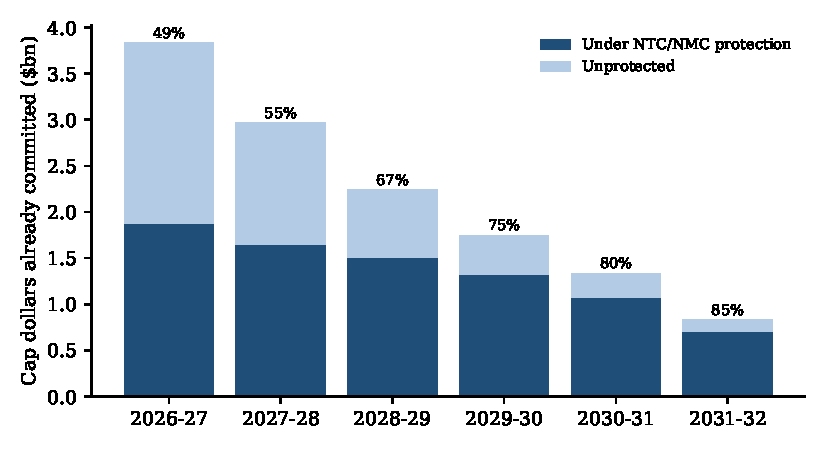
\includegraphics[width=0.75\linewidth]{../analysis/figures/fig_forward.pdf}
\caption{Cap dollars already committed for future seasons as of 30 October 2026, by protection status. Labels give the protected share of committed dollars.}\label{fig:forward}
\end{figure}

\begin{table}[t]\centering\small
\caption{The protection overhang: commitments already signed as of 30 October 2026}\label{tab:forward}
\begin{tabular}{lrrrrrr}\toprule
Season & Protected & NMC & Full NTC/NMC & Protected \$M & All committed \$M & Protected share\\\midrule
2026-27 & 306 & 120 & 170 & 1,871 & 3,834 & 0.49\\
2027-28 & 250 & 97 & 124 & 1,646 & 2,972 & 0.55\\
2028-29 & 220 & 73 & 91 & 1,504 & 2,242 & 0.67\\
2029-30 & 182 & 52 & 64 & 1,320 & 1,750 & 0.75\\
2030-31 & 138 & 36 & 38 & 1,072 & 1,338 & 0.80\\
2031-32 & 82 & 23 & 22 & 707 & 831 & 0.85\\
\bottomrule\end{tabular}
\end{table}

\subsection{Protection and the trade market}

\paragraph{Season-level patterns.} Across the 17 complete league years from 2009--10 to 2025--26, the protected share of cap dollars is positively correlated with total trade volume ($r=0.50$). That correlation disappears once the controls in Table~\ref{tab:season} are added: cap growth, the flat-cap years, shortened seasons, expansion-draft years and a linear trend. With 17 observations and trending series, the honest summary is that rising protection has not visibly reduced the overall volume of trades or of star trades. What it has changed is the \emph{composition} of trades. The share of trades that move a protected player tracks prevalence closely ($r=0.91$). It rose from roughly one in six in the 2010s to 30 per cent in 2024--25 and 26 per cent in 2025--26, and the relationship survives the controls (coefficient 1.34, $p<0.01$). A growing fraction of the league's transactions therefore pass through a player veto. Contemporary accounts of the quiet 2026 deadline say the same: vetoes, alongside new cap rules, kept several large deals from happening \citep{tsn_deadline2026}.

\begin{figure}[t]\centering
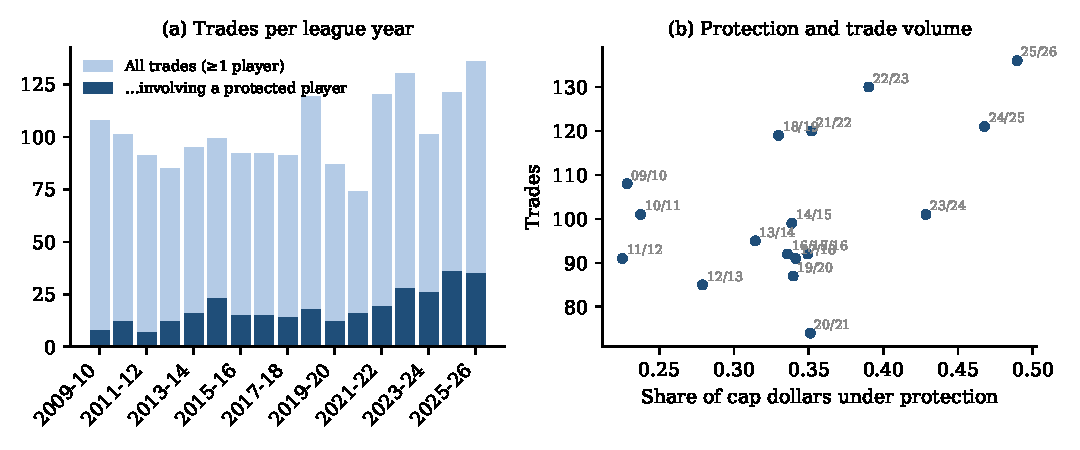
\includegraphics[width=\linewidth]{../analysis/figures/fig_trades.pdf}
\caption{Trades by league year and the share involving a protected player (a), and the protected share of cap dollars against trade volume (b), 2009--10 to 2025--26.}\label{fig:trades}
\end{figure}

\begin{table}[t]\centering\small
\caption{Season-level regressions, 2009--10 to 2025--26}\label{tab:season}
\begin{tabular}{lcccc}\toprule
 & All trades & Star trades & Deadline-day & Share w/ protected\\\midrule
Protected share of cap \$ & -40.14 & 42.45 & -40.95 & 1.34$^{*}$\\
 & (173.80) & (34.24) & (91.33) & (0.45)\\
Cap growth (pct.) & 71.80 & -11.12 & -31.41 & 0.05\\
 & (82.21) & (17.44) & (61.34) & (0.18)\\
Flat-cap era & 13.75 & 7.21 & -3.48 & 0.04\\
 & (10.20) & (3.75) & (8.20) & (0.03)\\
Shortened season & -27.05$^{*}$ & -5.53 & 0.12 & 0.01\\
 & (10.08) & (2.94) & (6.19) & (0.03)\\
Expansion draft year & -15.99$^{*}$ & -3.54 & -2.03 & -0.01\\
 & (5.09) & (2.06) & (4.30) & (0.01)\\
Linear trend & 2.07 & -0.70 & 1.00 & -0.01\\
 & (2.54) & (0.60) & (1.48) & (0.01)\\
Constant & 103.40$^{*}$ & -0.08 & 29.52 & -0.21$^{*}$\\
 & (43.55) & (7.46) & (21.44) & (0.10)\\
N & 17 & 17 & 17 & 17\\
$R^2$ & 0.75 & 0.80 & 0.21 & 0.88\\
\bottomrule\end{tabular}
\begin{minipage}{0.95\linewidth}\footnotesize\vspace{4pt}
\emph{Notes:} OLS with HC3 standard errors in parentheses; $^{*}p<0.05$. ``Star trades'' move at least one player whose cap hit is at least 7.5 per cent of the upper limit. ``Deadline-day'' trades are those on the busiest February--April date of each season, which coincides with the official deadline in every season checked. Shortened seasons: 2012--13, 2019--20, 2020--21. Expansion-draft years: the seasons on either side of the 2017 and 2021 expansion drafts.
\end{minipage}
\end{table}

\paragraph{Player-level trade hazards.} The cleaner test uses the player-season panel. Table~\ref{tab:hazard} estimates the probability that a player is traded in a given season, for players aged 26 or older earning at least three per cent of the cap, from 2013--14 to 2025--26. The controls are cap share, age, years remaining, position, prior-season scoring and season fixed effects. Unconditionally, 19.5 per cent of unprotected player-seasons in this group end in a trade, against 10.7 per cent of protected ones. Conditionally, a full NTC lowers the annual trade probability by about 7 percentage points and an NMC by about 8, against a mean of 14 per cent. These are reductions of roughly half. A modified NTC lowers it by only 3 points ($p\approx0.05$--$0.10$). Among stars, the NMC effect is the same size and is half of a smaller base rate. Clauses therefore do what they say: they keep players in place. But the protected players who \emph{are} traded are, by construction, traded on terms they accept. That is the condition under which the model predicts the seller's return collapses.

\begin{table}[t]\centering\small
\caption{Probability of being traded in a season, by clause type (2013--14 to 2025--26)}\label{tab:hazard}
\begin{tabular}{lcccc}\toprule
 & (1) LPM & (2) LPM & (3) LPM, stars & (4) Logit\\\midrule
Modified NTC & -0.030 & -0.026 & -0.050 & -0.173\\
 & (0.016) & (0.016) & (0.034) & (0.120)\\
Full NTC & -0.071$^{*}$ & -0.073$^{*}$ & -0.025 & -0.645$^{*}$\\
 & (0.019) & (0.019) & (0.042) & (0.224)\\
NMC & -0.081$^{*}$ & -0.082$^{*}$ & -0.082$^{*}$ & -0.855$^{*}$\\
 & (0.016) & (0.016) & (0.028) & (0.181)\\
Cap hit (share of cap) & 0.480 & 0.682 & 0.528 & 16.060\\
 & (1.081) & (1.105) & (4.333) & (12.272)\\
Points per game, prior season &  & -0.060$^{*}$ & -0.050 & -0.545$^{*}$\\
 &  & (0.025) & (0.033) & (0.244)\\
N (player-seasons) & 3947 & 3791 & 1049 & 3791\\
Mean of DV & 0.141 & 0.142 & 0.071 & 0.142\\
\bottomrule\end{tabular}
\begin{minipage}{0.95\linewidth}\footnotesize\vspace{4pt}
\emph{Notes:} Player-seasons for players aged 26 or older at the start of the season with a cap hit of at least 3 per cent of the upper limit. The omitted category is no clause. All models include age and its square, cap share squared, years-remaining indicators, a goaltender indicator and season fixed effects. Standard errors are clustered by player; $^{*}p<0.05$. Column (3) restricts to cap hits of at least 7.5 per cent. Column (4) reports logit coefficients.
\end{minipage}
\end{table}

\subsection{Is protection priced?}

Proposition~\ref{prop:price} predicts that a clause should be paid for with a lower wage, by an amount that rises with the perceived probability of a demand. Table~\ref{tab:hedonic} tests this on 496 new multi-year skater contracts signed by players aged about 26 or older, from 2009--10 to 2026--27. The dependent variable is the log of the first-season cap share. Controls are platform-season points per game (with a separate slope for defencemen), games played, age, log term and signing-year fixed effects. Protected contracts carry cap shares about 9 per cent \emph{higher}, not lower. Splitting by type, the premium sits entirely with full NTCs and NMCs. There is no sign that contracts signed in 2026--27 price protection differently, although that cohort is small.

The premium does not mean the clause is literally worth money to the team. Clauses go to players with bargaining power that the controls only partly capture, so the coefficient is an upper bound on any true compensating differential. A causal estimate would need an instrument, and the most promising candidate is the Article 11.8 eligibility threshold. The point is negative: there is no evidence of the discount the efficient-pricing benchmark requires. This contrasts with \citet{pedacehall2012} for baseball. Whether because general managers have underestimated $q$, or because the cap makes protection the cheapest currency available, teams have been granting vetoes without visibly charging for them. The 2026 wave is the event that should reprice them. Section~\ref{sec:implications} describes what repricing would look like.

\begin{table}[t]\centering\small
\caption{The price of protection: log first-season cap share on new skater contracts}\label{tab:hedonic}
\begin{tabular}{lccc}\toprule
 & (1) & (2) & (3)\\\midrule
Any protection & 0.086$^{*}$ & 0.027 & 0.086$^{*}$\\
 & (0.020) & (0.024) & (0.020)\\
Full NTC/NMC (vs. modified) &  & 0.097$^{*}$ & \\
 &  & (0.021) & \\
Any protection $\times$ signed 2026-27 &  &  & 0.008\\
 &  &  & (0.043)\\
Points/game, platform season & 0.558$^{*}$ & 0.540$^{*}$ & 0.558$^{*}$\\
 & (0.034) & (0.033) & (0.034)\\
log(term in seasons) & 0.304$^{*}$ & 0.268$^{*}$ & 0.304$^{*}$\\
 & (0.028) & (0.029) & (0.028)\\
Age at signing & -0.121 & -0.135$^{*}$ & -0.121\\
 & (0.064) & (0.063) & (0.064)\\
N (contracts) & 496 & 496 & 496\\
$R^2$ & 0.60 & 0.62 & 0.60\\
\bottomrule\end{tabular}
\begin{minipage}{0.95\linewidth}\footnotesize\vspace{4pt}
\emph{Notes:} New contracts with term of at least three seasons and a cap hit of at least 5 per cent of the upper limit, signed by players aged at least 25.5, 2009--10 to 2026--27; skaters with more than 20 platform-season games. All models include age squared, a defence indicator, its interaction with points per game, platform games played and signing-year fixed effects. HC3 standard errors; $^{*}p<0.05$. ``Any protection'' means any clause in any season of the contract.
\end{minipage}
\end{table}

\begin{figure}[t]\centering
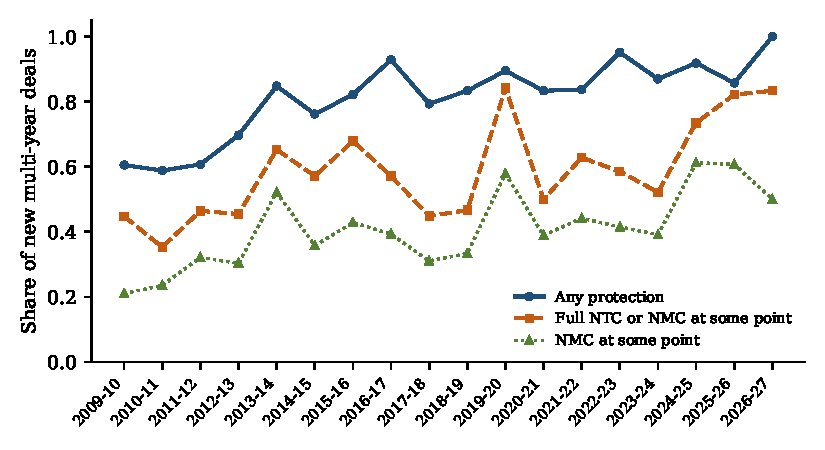
\includegraphics[width=0.75\linewidth]{../analysis/figures/fig_cohorts.pdf}
\caption{Protection in new multi-year contracts for established players, by signing year (term $\geq3$, cap hit $\geq5\%$, age $\geq25.5$). The 2026--27 cohort is partial (signings to 30 October 2026).}\label{fig:cohorts}
\end{figure}

\subsection{The case dataset}

To study what happens once a protected player wants out, I coded 25 cases between 2007--08 and 2026--27 (Appendix Table~\ref{tab:cases}). There are 16 player-initiated or mutual exits by protected players (including the ambiguous Luongo request and the disputed Kessel request), four exits by stars without a clause (Duchene, Dubois, Eichel and Hughes), and five protected stars who used their clause to stay, to choose a destination, or to veto a team-initiated deal without demanding out (Sundin, Marner, Iginla, Kane, and Werenski's reported veto). Each case records the request date and whether it was formal, informal, private or public, the clause, the number of approved destinations where reported, vetoes, days to resolution, and the return. The return is measured in two ways. The first is \emph{pick capital}, the sum of incoming draft picks valued with an empirical chart of expected career games by draft slot built from the 2005--14 drafts and normalised to the 16th pick (Appendix Figure~\ref{fig:pickvalue}). The second is \emph{realised games}, the NHL games that incoming players played in the three seasons after the trade, computed only for trades completed by 2023--24. Both measures are crude, and with this few cases they are best read as structured description.

The comparisons nonetheless line up with the model (Figure~\ref{fig:cases}). Protected demands returned less than unprotected ones on both measures: 0.84 against 1.27 mid-first-round equivalents in picks, and 263 against 354 realised games. They did not resolve faster (142 days against 170), which is consistent with clauses lowering the cost of waiting. Demands that were public from the start returned 0.44 mid-first equivalents in picks, against 1.48 for those that began privately, as Proposition~\ref{prop:audience} predicts. They also resolved faster (120 against 178 days), which is the point of going public. The realised-games measure points the other way, however: 309 games for public-from-the-start demands against 256 for those that began privately. The audience-cost result therefore rests on draft capital alone and should be treated as suggestive. Among protected cases with a reported list, the number of approved destinations is positively rank-correlated with realised games ($\rho=0.63$, $n=8$, $p=0.10$) but not with pick capital. Tkachuk's three first-round picks from a four-team list are the conspicuous outlier, discussed below.

\begin{figure}[t]\centering
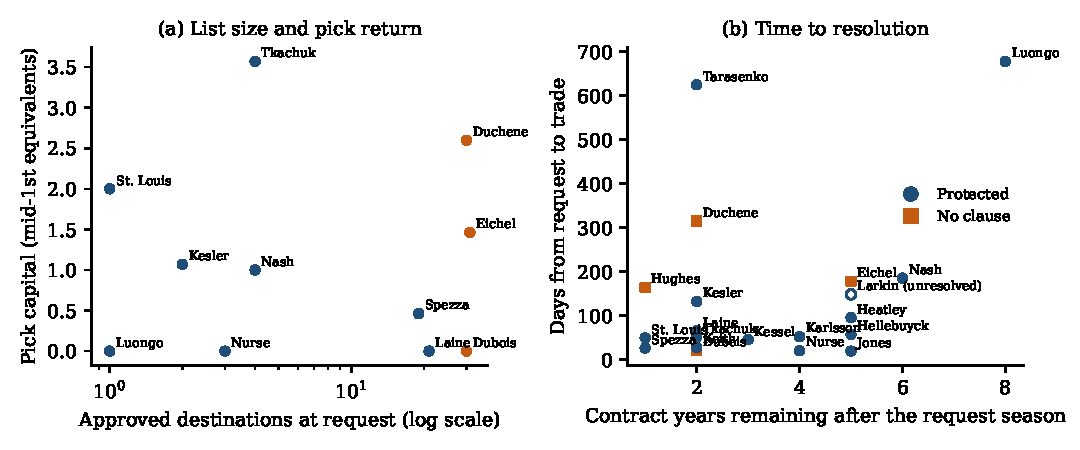
\includegraphics[width=\linewidth]{../analysis/figures/fig_cases.pdf}
\caption{Approved destinations and pick return (a), and contract years remaining and days to resolution (b), for trade demands 2009--2026. Larkin's request is unresolved (censored at 30 October 2026).}\label{fig:cases}
\end{figure}

\section{Case Studies}\label{sec:cases}

The four 2025--26 cases each isolate one mechanism of the model. Read together with three historical cases, they show how the mechanisms combine.

\subsection{Quinn Hughes: informal protection without a clause}

Hughes held no trade protection: his contract, which ran through 2026--27 at \$7.85 million, contained no clause \citep{cbs_hughes}. His agent says there was no formal trade request. What Vancouver had was a signal, given in the previous offseason, that a long-term extension was highly unlikely, and the trade followed from it \citep{espn_hughes}. Yet the agent described Vancouver's conduct this way: the club worked with the player ``as if we had a no-trade clause, almost'' \citep{dailyhive_hughes}. This is Proposition~\ref{prop:informal} in action. With eighteen months left on his deal, most of Hughes's value to an acquirer lay in the right to extend him, and that right was worth something only to teams he would agree to re-sign with. Selling to anyone else would have been selling a rental. The return was large: two young NHL roster players (Marco Rossi and Zeev Buium), a prospect (Liam \"Ohgren) and a first-round pick. That fits the model's claim that informal protection narrows the effective market without eliminating competition among the approved buyers. The postscript fits too. As of late October 2026, Hughes had not extended with Minnesota and was reported to prefer a short term \citep{rmnb_hughes}. The extension option Minnesota bought remains unexercised.

\subsection{Brady Tkachuk: the veto player who still got a price}

Tkachuk held a full NMC with two seasons left at \$8.2 million. Accounts differ on how his exit began. On the night of the trade, one outlet reported that ``a formal trade request may not have been made,'' only an unwillingness to extend \citep{fourthperiod_tkachuk}. The next day general manager Steve Staios said that ``what changed was a trade request,'' and Tkachuk confirmed he had asked out: ``It wasn't an easy decision'' \citep{yahoo_staios,thescore_tkachuk}. What remains disputed is when the decision was made, since Tkachuk had publicly called the rumours ``just not true'' in April. Staios was explicit about the clause's effect: ``The dynamic of a no-trade clause changes how the transaction works and how it's going to look\ldots It's not like he was available to every team in the league.'' The process was ``clearly pointed at one team at the end'' \citep{yahoo_staios,tsn_staios}. Tkachuk's reported list had four teams: Florida, Minnesota, Vegas and Carolina.

The model predicts a poor return when $m$ is effectively one, yet Ottawa received the ninth and 25th picks in the 2026 draft, a top-ten-protected 2029 first and a 2027 second \citep{fourthperiod_tkachuk}. That is the largest pick package in the dataset. Two features of the model reconcile the outcome. First, Ottawa's retention value was high. Tkachuk was under contract for two more seasons, the request was private until after the trade, and Ottawa plausibly could have kept him into the season. Under the outside-option logic of Section~\ref{sec:model}, a credible threat to keep the player sustains the price even in bilateral bargaining. Second, Florida's valuation was unusually high, because it was the only approved team that could pair Brady with his brother Matthew. A single buyer with a very high $v$ can pay a lot even when $T$'s share of the surplus is modest. The Tkachuk case is therefore not evidence against the veto mechanism. It is evidence that the mechanism operates on the seller's \emph{share}, and that the share can be protected by keeping the request private.

\subsection{Dylan Larkin: stalemate and sunk costs}

Larkin asked Detroit to trade him on 4 June 2026, with five seasons remaining at \$8.7 million on an eight-year contract he had signed as captain in 2023 \citep{wilx_larkin,nhl_larkin}. His initial list had three teams: Minnesota, Florida and Vegas. In the model's terms $m=3$, the region of Table~\ref{tab:model} where the seller loses roughly half the competitive price. Proposition~\ref{prop:delay} predicts delay in exactly these conditions, because a narrow list lowers the value of selling now relative to waiting. Delay is what followed.

Detroit's general manager, Steve Yzerman, was removed on 15 July. Shawn Horcoff was named interim general manager on 15 September \citep{nhl_horcoff}. Larkin was stripped of the captaincy, booed at the home opener, and placed on non-roster injured reserve, with the coach remarking that ``he's got to live with the ramifications of asking for a trade'' \citep{espn_larkin_ir}. The list expanded under pressure, to ten teams by late October \citep{dfo_larkin_list}. In the model this is $m$ rising over time, and it is the player, not the clause, that relaxes the constraint. On 29 October, after Larkin's agent said he would not report, Detroit suspended him without pay. Horcoff said the club would ``continue to explore trade opportunities,'' but only in ``the best interests of the Detroit Red Wings'' \citep{cod_larkin_suspended}. Suspension is the team's counter-move. It cannot remove the veto, but it raises the player's cost of waiting, which pushes him to widen the list.

Larkin is also the cleanest example of the sunk-cost temptation in Proposition~\ref{prop:delay}(c). A team that has committed \$69.6 million to its captain and built its rebuild around him has every reason to believe the relationship can be repaired, that is, to overestimate $\rho$. Detroit's first moves (waiting, then a leadership change) look like a bet on reconciliation. Its later moves (stripping the captaincy, the suspension) look like the recognition that $\rho$ had fallen to zero. At the time of writing the spell is censored at 148 days and counting.

\subsection{Connor Hellebuyck: audience costs}

Hellebuyck held an NMC with five seasons remaining at \$8.5 million. He asked for a trade privately early in the 2026 offseason. On 27 August he made the request public in a statement posted by his agent \citep{tsn_hellebuyck_open}. When he did not report to camp, Winnipeg suspended him on 16 September. General manager Kevin Cheveldayoff insisted that ``a contract is a contract'' \citep{nhl_hellebuyck_suspended}. Buffalo pursued him for weeks without a deal. On 23 October Winnipeg traded him to New Jersey for forward Dawson Mercer, the veteran Nick Bjugstad, goaltender Nico Daws, the rights to prospect Alexander Command, a 2029 second-round pick and a 2027 seventh \citep{nhl_hellebuyck_trade,tsn_hellebuyck_trade}.

The sequence follows the logic of equation~\eqref{eq:public}. While the request was private, Winnipeg could plausibly tell suitors it was prepared to keep the reigning Olympic best goaltender, so $R$ was high and selling was not urgent. Going public, then refusing to report, lowered $\lambda$ to zero and with it $R$. That made the exit credible and the sale inevitable. Unlike Larkin, Hellebuyck was reportedly open to a broad range of destinations \citep{thw_larkin_hellebuyck,tsn_hellebuyck_open}. Proposition~\ref{prop:audience} says the cost of publicity is smallest when $m$ is large, and the return was a useful but unspectacular package of roster players with no first-round pick. That is about what the model predicts for a seller with no outside option and a moderately competitive market.

\subsection{Historical cases}

\paragraph{Dany Heatley (2009): the veto exercised.} Heatley asked Ottawa to trade him in June 2009, with five years left on a six-year, \$45 million contract. When Ottawa agreed a deal with Edmonton for Andrew Cogliano, Dustin Penner and Ladislav \v{S}m\'{i}d, he refused to waive \citep{heatley_thn}. Ottawa settled for Milan Michalek, Jonathan Cheechoo and a second-round pick from San Jose in September. The case shows that the veto does more than shrink the market ex ante. It also lets the player reject a completed negotiation, which hands the remaining buyers knowledge of the seller's weakened position.

\paragraph{Martin St. Louis (2014): one destination.} St. Louis asked Tampa Bay privately in January 2014 and would accept only the Rangers \citep{stlouis_cbs}. With $m=1$, Tampa Bay's return was Ryan Callahan, a pending free agent, plus first-round picks. This is the bilateral case of the model, with a seller whose retention value of an aging star at the deadline was modest.

\paragraph{Roberto Luongo (2012--14): recapture.} Luongo's twelve-year contract and NTC, combined with a public willingness to move only to Florida, produced a stalemate of almost two years \citep{luongo_nesn}. Vancouver eventually moved him to Florida for a young goaltender, Jacob Markstr\"om, and a forward, Shawn Matthias. The long contract made the recapture liability enormous, which deterred buyers. The narrow list removed competition, and Vancouver's preference to wait for a better market cost it the asset's value. This is the longest-duration resolved case in the data and the clearest historical analogue for Larkin.

\paragraph{The counterfactuals.} Matt Duchene and Jack Eichel, the two most prominent unprotected stars who wanted out, also produced long standoffs (315 and 178 days). But their teams eventually ran open, competitive auctions and extracted large returns \citep{eichel_ap}. Duchene's three-team deal yielded Samuel Girard, prospects, and an Ottawa first that became the fourth overall pick. The absence of a veto did not prevent delay. It did preserve competition.

\section{Implications for Contract Design}\label{sec:implications}

If the 2026 wave raises the perceived probability of demands ($q$), Proposition~\ref{prop:price} predicts that protection will be repriced. The model also says which features of a clause matter most, so it predicts the form the repricing should take.

\begin{enumerate}[leftmargin=*,itemsep=2pt]
\item \textbf{Ban lists that are too short, not lists themselves.} Because order statistics flatten quickly, a no-trade list that leaves 15 or 20 approved teams costs the team almost nothing on exit. A trade list naming three costs it most of the value. The efficient contract caps the player's veto at a minimum approved set (for example, at least eight teams). It does not have to deny protection altogether.
\item \textbf{Schedule the clause to decay.} Converting an NMC into a modified NTC on a fixed date, and having lists shrink over time, raises $m$ in later years. That makes waiting less attractive to the player and selling more attractive to the team (Proposition~\ref{prop:delay}). Many recent contracts already do this, and more should.
\item \textbf{Stagger clause dates across the roster.} A team whose stars' protection windows open and close together has no flexibility in a crisis. Staggering keeps some assets always tradable.
\item \textbf{Price the clause explicitly.} The absence of a measurable wage discount (Section~\ref{sec:empirics}) suggests that teams have treated protection as free. A team that values the option to sell should demand cap savings for an NMC, or offer an NMC only in the years when demands are least likely.
\item \textbf{Keep requests private.} Since audience costs destroy the seller's outside option only when the approved list is short, teams have the strongest interest in confidentiality exactly when a player names few teams. A protocol committing both sides to a private negotiation window before any public statement would protect the seller's surplus without removing the player's right.
\item \textbf{Bargain over it at the league level.} Bettman's remark makes clear that the clause will be on the agenda for the next CBA. The model suggests a reform that protects the players' interest in stability while restoring competition at exit. One example: a league-wide minimum for the size of approved lists after a player-initiated request. It need not restrict clause eligibility.
\end{enumerate}

The argument also generalises beyond hockey. Any veto right granted to protect a weaker party in a long-term relationship can, once the relationship sours, become an instrument with which that party, or the third party it favours, extracts surplus. Examples include consent rights in joint ventures, anti-dilution and tag-along rights for minority investors, and alliance commitments that require partner approval before forces move. In each case the right is ex ante protective and ex post extractive. In each case the design remedy is the one proposed here: limit how far the veto can narrow the field, not whether the veto exists.

\section{Conclusion}\label{sec:conclusion}

A no-trade clause is a promise made by a team to a player. A long-term contract is a promise made by a player to a team, but only the first promise is enforceable. When the second fails, the first becomes a weapon. The protected player can name his buyers, signal that the seller must sell, and, by going public, destroy the seller's last threat. The surplus that changes hands goes not to the player but to the team he chooses.

The data show that the NHL has moved steadily into the region where this matters. Nearly half of all cap dollars, more than three-quarters of star contracts, and a rising share of future commitments now carry a veto. Protection keeps players in place, roughly halving the annual chance that a protected player is traded. But a growing share of trades now pass through those vetoes, and protection has not been priced. The theory predicts the response: narrower vetoes, decaying clauses, explicit prices, and a fight at the next bargaining table. Whether the 2026 wave produces that response is the natural test of the argument, and the data assembled here make it possible to run.


\bibliography{references}
\appendix
\section{Proofs}\label{app:proofs}

Throughout, $F$ has support $[0,\bar v]$ and positive density, and $G_{(2:m)}(y)=F(y)^m+mF(y)^{m-1}(1-F(y))$ is the probability that at most one of $m$ valuations exceeds $y$, i.e.\ the CDF of $v_{(2:m)}$.

\paragraph{Proof of Proposition~\ref{prop:veto}.} (i) For $m\ge2$, $\Pi(m,R)=\mathbb{E}[\max\{v_{(2:m)},R\}]=R+\int_R^{\bar v}\big(1-G_{(2:m)}(y)\big)\,dy$. Adding a bidder can only add values above $y$, so ``at most one of $m+1$ exceeds $y$'' implies ``at most one of the first $m$ exceeds $y$''. Hence
\begin{align*}
G_{(2:m)}(y)-G_{(2:m+1)}(y)&=\Pr(\text{exactly one of the first $m$ exceeds $y$, and so does the new one})\\
&= mF(y)^{m-1}(1-F(y))^2 ,
\end{align*}
which is strictly positive on $(0,\bar v)$. So $\Pi(m+1,R)-\Pi(m,R)=\int_R^{\bar v}mF^{m-1}(1-F)^2\,dy>0$ whenever $R<\bar v$. Monotonicity in $k$ follows from $m=N-k$.
(ii) The increment $\Delta(m)=\int_R^{\bar v}mF^{m-1}(1-F)^2dy$ tends to zero as $m\to\infty$ by dominated convergence, because $mF^{m-1}\to0$ pointwise on $F<1$. For $F=U[0,1]$ and $R=0$, $\mathbb{E}[v_{(2:m)}]=(m-1)/(m+1)$, so $\Delta(m)=2/((m+1)(m+2))$, which is strictly decreasing.
(iii) For $U[0,1]$ and $R=0$, $\Pi(1)=\beta\,\mathbb{E}[v]=\beta/2$ and $\Pi(2)=\mathbb{E}[\min(v_1,v_2)]=1/3$. Hence $\Pi(2)>\Pi(1)$ if and only if $\beta<2/3$. $\square$

\paragraph{Proof of Proposition~\ref{prop:audience}.} (i) For $m\ge2$, differentiating $R+\int_R^{\bar v}(1-G_{(2:m)})$ gives $1-(1-G_{(2:m)}(R))=G_{(2:m)}(R)>0$ for $R>0$. For $m=1$, $\Pi=R+\beta\int_R^{\bar v}(1-F)$, so $\partial\Pi/\partial R=1-\beta(1-F(R))>0$ when $\beta<1$ or $F(R)>0$. Because $R_{\text{pub}}<R_{\text{priv}}$ by (\ref{eq:R}) and $\lambda_{\text{pub}}<\lambda_{\text{priv}}$, $\Pi(m,R_{\text{pub}})<\Pi(m,R_{\text{priv}})$.
(ii) The loss from publicity is $L(m)=\int_{R_{\text{pub}}}^{R_{\text{priv}}}\partial\Pi/\partial R\,dr$. For $m\ge2$ the integrand $G_{(2:m)}(r)$ is strictly decreasing in $m$ by the argument in (i) above, so $L(m)$ is strictly decreasing. Comparing $m=1$ and $m=2$: $1-\beta(1-F)\ge 1-(1-F)^2=G_{(2:2)}$ if and only if $\beta\le 1-F$, which holds on $[R_{\text{pub}},R_{\text{priv}}]$ when $\beta\le 1-F(R_{\text{priv}})$. $\square$

\paragraph{Outside-option refinement.} In Rubinstein alternating offers between $T$ and a single acquirer with discount factors $\delta_T,\delta_A$, and with $T$ able to opt out to $R$ at any point, the unique subgame-perfect payoff to $T$ is $\max\{\beta^\ast v,R\}$, where $\beta^\ast=(1-\delta_A)/(1-\delta_T\delta_A)$ \citep{rubinstein1982,bss1989}. A fall in $R$ therefore changes $T$'s payoff only when $R>\beta^\ast v$.

\paragraph{Proof of the publicity condition (\ref{eq:public}).} $P$'s expected payoff from signal $s$ is $\tau_s u_{\text{out}}+(1-\tau_s)\big[u_{\text{stay}}-c_P\,\mathbf{1}\{s=\text{pub}\}\lambda_s\big]$, where the audience cost is paid only if he reconciles. The cost $c_P$ enters through $\lambda_{\text{pub}}$, the probability of the reconciliation that would trigger it; to a first approximation it is incurred with that probability. Rearranging the comparison gives (\ref{eq:public}). With $m\ge2$, $\tau_s=1-F(R_s)^m$, which is decreasing in $R_s$, so $\tau_{\text{pub}}>\tau_{\text{priv}}$. $\square$

\paragraph{Proof of Proposition~\ref{prop:delay}.} Selling now yields $\Pi(m,R)$. Waiting yields $V=1$ with probability $\rho$, and otherwise the discounted sale value $\delta\Pi(m',R')$. The comparison is immediate. Since $\Pi$ is increasing in $m$, a low current $m$ lowers the left-hand side of the sell-now comparison, and $m'>m$ raises the value of waiting. $\square$

\paragraph{Proof of Proposition~\ref{prop:price}.} Let $U_P=w+B(k)$ and $U_T=Y-w-C(k)$, with disagreement payoffs $\underline U_P,\underline U_T$. Generalised Nash bargaining with transferable utility gives $U_P-\underline U_P=\alpha S(k)$, where $S(k)=Y+B(k)-C(k)-\underline U_P-\underline U_T$. Solving, $w(k)=\underline U_P+\alpha S(k)-B(k)$, so $w(k)-w(0)=-(1-\alpha)B(k)-\alpha C(k)$ (normalising $B(0)=C(0)=0$). Then $\partial w/\partial k=-(1-\alpha)B'(k)-\alpha C'(k)$, and $C'(k)=q\,\partial[\Pi(N,R)-\Pi(N-k,R)]/\partial k+C_0'(k)$ rises with $q$ because $\Pi$ is increasing in $m$. If $w$ is constrained from below, the first-order condition for $k$ ($B'=C'$) holds with $C'$ increasing in $q$, so the chosen $k$ falls as $q$ rises. $\square$

\paragraph{Proof of Proposition~\ref{prop:informal}.} Approved acquirers value $P$ at $x_i+E>\bar x\ge x_j$ for every unapproved $j$. With $|A|\ge2$, the two highest valuations among all $N$ acquirers therefore both belong to $A$. The competitive price is the second-highest approved valuation, exactly as in a sale restricted to $A$. Because $x_i$ is increasing in the remaining term $\tau$, $\bar x(\tau)$ is increasing in $\tau$, so the condition $E>\bar x(\tau)$ is easier to satisfy near the end of a contract. $\square$

\section{Data Appendix}\label{app:data}

\paragraph{Sources.} Contracts and transactions: CapWages player pages (\url{https://capwages.com/players/*}), all 7,971 slugs in the site's sitemap, collected 30 October 2026; 7,965 returned data (script \path{analysis/02_fetch_capwages.py}). Rosters for coverage checks: NHL public API, \path{api-web.nhle.com/v1/roster/<team>/<season>} (script \path{01_fetch_rosters.py}). Salary cap: NHL CBA and league announcements (\path{data/salary_cap_by_season.csv}). The 2012--13 figure is the \$70.2 million full-season-equivalent limit rather than the nominal \$60 million. Deadline-day counts: NHL Stats Pack \citep{nhl_statspack}. Cases: news reports cited row by row in \texttt{data/protected\_player\_cases.csv}.

\paragraph{Key variables.}
\begin{description}[leftmargin=1em,itemsep=1pt,font=\normalfont\itshape]
\item[clause] The strongest protection listed for the contract-season: NMC $>$ M-NMC $>$ NTC $>$ M-NTC $>$ none.
\item[list\_n, list\_type] The first list size parsed from the clause text. ``block'' means a no-trade list (teams the player may refuse); ``approve'' means a trade list (teams he would accept). The parse is approximate where lists change by season.
\item[protected trade] A trade, identified by a CapWages trade ID, that moved at least one player whose contract carried any clause in that league year.
\item[star] A cap hit of at least 7.5 per cent of the upper limit in that season.
\item[deadline day] The February--April date with the most trades in the league year. It matches the official deadline date in every season from 2008--09 to 2025--26.
\item[pick value] Expected career NHL games by overall pick, from the 2005--14 drafts. A pick whose player never played, or is absent from the archive, counts as zero. Values are smoothed with $\hat g(p)=a(p+c)^{-b}+d$ and normalised to pick 16. Pick slots that are not yet known are set to 16 (first round), 48 (second), 80 (third), 112 (fourth) and 208 (seventh).
\item[realized\_gp\_3yr] Regular-season NHL games played by players received, in the league year of the trade and the two following.
\end{description}

\paragraph{Known gaps.} Coverage is incomplete before 2013--14 (Section~\ref{sec:empirics}). Pick-only trades are excluded from trade counts. Clause types are as reported by CapWages and were not independently audited contract by contract. Request dates in several cases are approximate, and the case file flags each one. See \texttt{METHODS\_NOTES.md} for the full list.

\begin{figure}[h]\centering
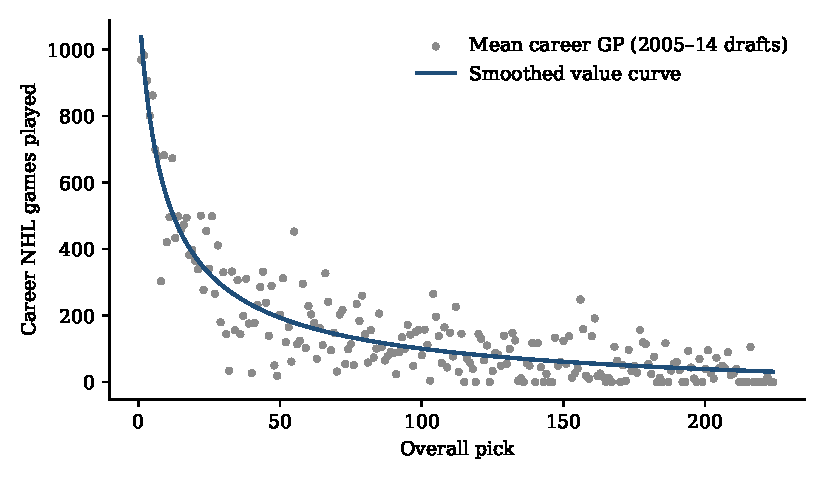
\includegraphics[width=0.7\linewidth]{../analysis/figures/pick_value.pdf}
\caption{Empirical draft-pick value chart: mean career NHL games by overall pick, 2005--14 drafts, with fitted curve.}\label{fig:pickvalue}
\end{figure}

\clearpage\section{Case Table}\label{app:cases}
\begin{table}[h]\centering\scriptsize
\caption{Star exits, demands and refusals, 2007--08 to 2026--27}\label{tab:cases}
\resizebox{\linewidth}{!}{\begin{tabular}{llllrrrrl}\toprule
Player & Team & Season & Clause & $m$ & Days & Picks & GP3 & Outcome\\\midrule
Mats Sundin & TOR & 2007-08 & NMC &  &  &  &  & stayed; signed with VAN as UFA\\
Dany Heatley & OTT & 2009-10 & NTC &  & 95 & 0.46 & 270 & SJS\\
Rick Nash & CBJ & 2011-12 & NMC & 4 & 185 & 1.00 & 395 & NYR\\
Jarome Iginla & CGY & 2012-13 & NTC &  &  & 0.70 & 24 & PIT\\
Martin St. Louis & TBL & 2013-14 & NMC & 1 & 49 & 2.00 & 215 & NYR\\
Roberto Luongo & VAN & 2013-14 & NTC & 1 & 678 & 0.00 & 278 & FLA\\
Ryan Kesler & VAN & 2013-14 & NTC & 2 & 132 & 1.07 & 362 & ANA\\
Jason Spezza & OTT & 2014-15 & M-NTC & 19 & 26 & 0.46 & 259 & DAL\\
Matt Duchene & COL & 2017-18 & none & 30 & 315 & 2.60 & 290 & OTT\\
Phil Kessel & PIT & 2018-19 & M-NTC &  & 45 & 0.00 & 181 & ARI\\
Pierre-Luc Dubois & CBJ & 2020-21 & none & 30 & 21 & 0.00 & 363 & WPG\\
Duncan Keith & CHI & 2021-22 & NMC &  & 27 & 0.29 & 149 & EDM\\
Jack Eichel & BUF & 2021-22 & none & 31 & 178 & 1.46 & 410 & VGK\\
Vladimir Tarasenko & STL & 2022-23 & NTC &  & 625 & 1.21 & 124 & NYR\\
Patrick Kane & CHI & 2022-23 & NMC & 2 &  & 0.67 & 0 & NYR\\
Erik Karlsson & SJS & 2023-24 & NMC &  & 52 & 1.00 & 399 & PIT\\
Patrik Laine & CBJ & 2024-25 & M-NTC & 21 & 65 & 0.00 &  & MTL\\
Seth Jones & CHI & 2024-25 & NTC &  & 19 & 1.00 &  & FLA\\
Mitch Marner & TOR & 2024-25 & NMC &  &  & 0.00 &  & VGK\\
Quinn Hughes & VAN & 2025-26 & none &  & 164 & 1.00 &  & MIN\\
Brady Tkachuk & OTT & 2025-26 & NMC & 4 & 51 & 3.57 &  & FLA\\
Dylan Larkin & DET & 2026-27 & NTC & 3 $\to$ 10 & 148+ &  &  & unresolved\\
Darnell Nurse & EDM & 2026-27 & NMC & 3 $\to$ 4 & 20 & 0.00 &  & SJS\\
Zach Werenski & CBJ & 2026-27 & NMC &  &  &  &  & stayed\\
Connor Hellebuyck & WPG & 2026-27 & NMC &  & 57 & 0.55 &  & NJD\\
\bottomrule\end{tabular}}
\begin{minipage}{0.97\linewidth}\footnotesize\vspace{4pt}
\emph{Notes:} $m$ is the reported number of approved destinations, where known. For Spezza and Laine it is computed from a ten-team no-trade list. Days run from the request, or from the public statement when the private date is unknown, to the trade; ``+'' marks a censored spell. Picks is incoming pick capital in mid-first-round equivalents. GP3 is the games played by incoming players over three seasons, shown for trades completed by 2023--24. Full sourcing, request types and conflicting accounts are recorded in \texttt{data/protected\_player\_cases.csv}.
\end{minipage}
\end{table}

\end{document}
